\documentclass[fr]{../../../eplsummary}
\usepackage{graphicx}
\usepackage[toc,page]{appendix} 
\usepackage{eurosym}
\usepackage{gensymb}
\usepackage{multirow}
\usepackage{chemfig}
\usepackage{tikz}
\usepackage{pgfplots}
\usepackage{pgffor}
\usepackage{qtree}

\usepackage{../../../eplchem}

\hypertitle{Projet}{3}{FSAB}{1503}
{Luca Derumier \and Marie-Ombeline Wilmet}
{Juray de Wilde}

\newpage

\section{Introduction}
\par Ce document est basé sur le projet P3 de l'année académique 2016-2017, il pourrait donc ne plus être valable pour les autres années. L'examen pourra prendre la forme de QCM, problème impliquant le calcul de valeurs numériques, question ouverte. L'examen écrit vise à évaluer la compréhension par l'étudiant des notions scientifiques et techniques, qui seront détaillées dans ce document, ainsi que son aptitude à les utiliser pour résoudre des problèmes ou analyser un cas concret.

Les équations et valeurs utiles seront fournies, il ne sera pas demandé de les restituer.

\section{Thématique 1 : Introduction au génie chimique}

\subsection{Procédé continu, démarrage et phase transitoire}

\par Le première thématique portait sur le laboratoire "grenadine" où nous avions dû réaliser un procédé continu qui comporte trois étapes : le démarrage, la phase transitoire et le régime stationnaire.
\begin{center}
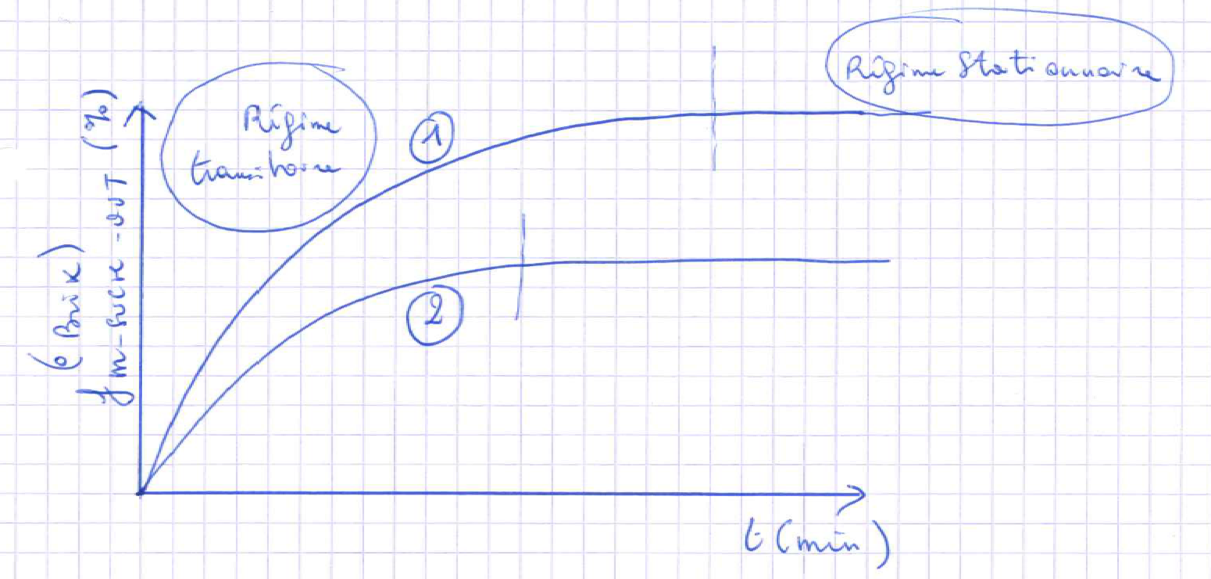
\includegraphics[scale = 0.3]{gren.png}
\end{center}

\subsection{Mesure de débits}
\par Le débit est la quantité de matière (exprimée par une masse ou un volume) qui passe à chaque unité de temps à travers cette section.

$$\dot{m} = \frac{\Delta m}{\Delta t} \,  [\frac{kg}{s}]$$

$$\dot{V} = \frac{\Delta V}{\Delta t} \,  [\frac{m^{3}}{s}]$$

\subsection{Bilan de matière en terme de débits massiques ou molaires}
\textbf{Bilan de matière :} calcul sur les débits, découlant du principe de conservation de la masse : "en régime stationnaire, la masse totale qui entre dans le réacteur, par unité de temps, est égale à la masse totale qui en sort". Ce calcul peut être effectué globalement sur les flux totaux (débit massique total), ou en considérant les flux des différents composés (l'eau, le sucre,...) ou même sur les flux des espèces atomiques (H,C,...)\\
\newline \textbf{Bilan de masse :} Pour pouvoir effectuer un bilan de masse, nous avons mesuré les masses volumiques de la grenadine, de l'eau et du mélange obtenu à la fin de l'expérience au laboratoire

\subsubsection{Régime stationnaire}

\par On peut vérifier le bilan de masse en régime stationnaire. Dans le cadre de la 

thématique 1 on avait :

\begin{itemize}
    \item $C_{x}$ la concentration du composant $x$ en fonction du temps en $[ \frac{kg}{L}]$ 
    \item $f_{m-x} = \frac{m_{x}}{m_{tot}}$ la fraction massique du composant $x$ dans la solution finale.
    \item $\Rightarrow C_{sucre-out} = f_{m-sucre-out} \, . \, \rho_{out}$ avec $\rho$ la masse volumique (attention à adapter les unités en fonction du problème, la masse volumique ayant les unités $[\frac{kg}{m^{3}}]$)
    \item 2 composants considérés : sucre et $H_{2}0$
    \item 2 flux entrants : Conc (Sirop Concentré) et Eau
    \item 1 flux sorant : Out\\

\end{itemize}
\par En régime stationnaire ($t=\infty$) on a donc :

$$\mbox{Débit massique entrant}=\mbox{Débit massique sortant}  $$
$$\dot{m}_{sucre-conc} = \dot{m}_{sucre-out}$$

$$\dot{V}_{conc} \, . \, c_{sucre-conc} = \dot{V}_{out} \, . \, c_{sucre-out} $$

\par On peut poser en $T=\infty$ : \\
$$\dot{V}_{in-total} = \dot{V}_{eau} + \dot{V}_{conc} = \dot{V}_{out}$$

$$\Rightarrow C_{out} = C_{sucre-conc} \, . \, \frac{\dot{V}_{conc}}{\dot{V}_{conc} + \dot{V}_{eau}}$$

$$\Leftrightarrow \frac{C_{sucre-out}}{C_{sucre-conc}} = \frac{\dot{V}_{conc}}{\dot{V}_{out}}$$

$$\Leftrightarrow \frac{f_{m-sucre-out}}{f_{m-sucre-conc}} = \frac{\dot{m}_{conc}}{\dot{m}_{out}}$$
 
\subsubsection{Phase transitoire}

\par Durant la phase transitoire, la concentration en sucre augmente dans le réacteur et donc dans le flux de sirop dilué.\\

$$C_{sucre-out} = c_{sucre-conc} \, . \, \frac{\dot{V}_{conc}}{\dot{V}_{conc} + \dot{V}_{eau}} \, . \, (1-e^{-t/\tau})$$

\par Avec $\tau = \frac{V_{R}}{\dot{V}_{out}}$ et $V_{R}$ le volume du réacteur (contenu). Si on veut vraiment se convaincre de l'origine de cette formule on peut voir qu'elle est en fait simplement la solution de l’équation différentielle suivante, qui décrit l’évolution du contenu du réacteur : 

$$\frac{\mathrm{d} C_{sucre-out}(t)}{\mathrm{d}t} = \frac{1}{V_{R}}(\dot{m}_{sucre-in}(t) - \dot{m}_{sucre-out}(t))$$
$$\Leftrightarrow \frac{\mathrm{d} C_{sucre-out}(t)}{\mathrm{d}t} = \frac{1}{V_{R}}(\dot{v}_{conc} \, C_{sucre-conc}(t) - \dot{v}_{out} \, C_{sucre-out}(t))$$

\par avec la condition limite $C_{sucre-out}(t=0) = 0$

\subsection{Questions Janvier 2016}
\textbf{La position des tuyaux était supposée fixe, comment avez-vous fait pour obtenir un débit $q_{out}$ constant ?} \\ Nous avons maintenus constants les débits d'alimentation en maintenant constants les niveaux $h_{R-E}$ et $h_{R-S}$ dans les réservoirs d'eau et de sirop ($h_{out}$ étant fixés) \\
\newline \textbf{Si le schéma à la page suivante respecte les distances, à quoi voit-on que les deux fluides eau et sirop concentré n'ont pas la même viscosité ?} \\ Les tuyaux d'alimentation en eau et en sirop ont le même diamètre et la différence de pression hydrostatique ($h_R - h_{out}$) est presque semblable dans les siphons d'eau et de sirop, alors que le débit d'eau est 4 fois plus important que le débit de sirop. On en déduit que l'écoulement du sirop nécessite une pression nettement supérieure à celle exigée  pour l'écoulement de l'eau, et donc une différence de viscosité des deux liquides. \\
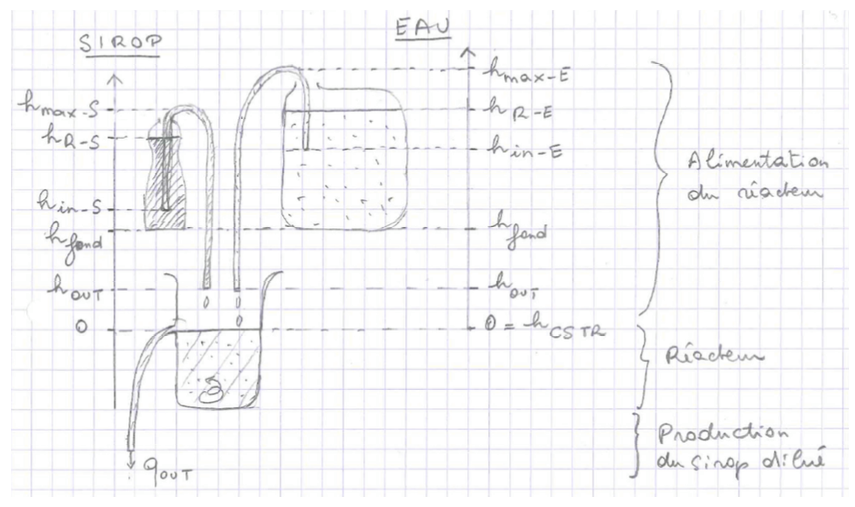
\includegraphics[width=15cm]{Schema_Labo_CSTR}\\
\newline \textbf{Pour changer la concentration finale en sucre dans le sirop dilué, je peux modifier (sans rien changer d'autre au schéma) (VRAI - FAUX)} \\ a. $h_{R-E}$ ou $h_{out}$ \\ VRAI : la différence de pression hydrostatique est donnée par $h_R - h_{out}$. Changer un de ces paramètres change donc le rapport entre les débits d'alimentation. \\ b. diamètre du tuyau de sortie ($q_{out}$) ou volume de réacteur \\ FAUX : la concentration en sortie dans le débit de sortie $q_{out}$ est déterminée à l'état stationnaire, par le rapport des débits d'alimentation en eau et sirop concentré, quel que soit le réacteur. \\ c. $h_{max-S}$, $h_{in-E}$ ou $h_{CSTR}$ \\ FAUX : tant que le siphon est amorcé, ces paramètres n'ont pas d'incidence sur l'alimentation en sirop et en eau. \\ 
\newline \textbf{En se basant sur le graphe ci-dessous et le schéma du montage ci-haut, on peut déduire que (VRAI-FAUX)} \\
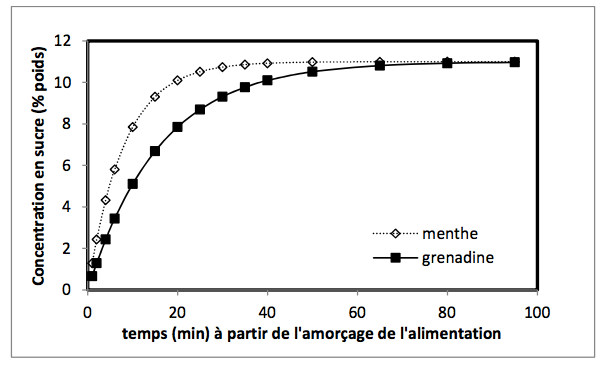
\includegraphics[width=15cm]{Graphe_Labo_CSTR}\\
a. le volume du réacteur "menthe" est plus grand que le volume du réacteur "grenadine" \\ FAUX : la phase transitoire est plus courte dans le cas "menthe" : le temps de séjour est donc plus court dans ce cas; les débits d'alimentation étant identiques; le volume du réacteur "menthe" est donc plus petit. \\ b. le volume du réacteur influence le débit de sortie $q_{out}$ \\ FAUX : cette affirmation n'a rien à voir avec le graphe; elle est par ailleurs erronée (voir question précédente) \\
\newline \textbf{Parmi les questions suivantes, laquelle/lesquelles est/sont vraie(s) ?} \\ a. à l'état stationnaire, le taux de sucre dans le flux de sortie sera environ égal à 1/4 du taux de sucre dans la bouteille de sirop. \\ FAUX : le débit d'alimentation en sirop est égal à 1/4 du débit d'alimentation en eau et est donc égal à 1/5 du débit total d'alimentation; le sirop sera donc dilué d'un facteur 5 \\ b. dans le montage CSTR représenté à la figure 3, la durée de la phase transitoire dépend de la concentration de sucre dans le flux d'alimentation \\ FAUX : la durée da la phase transitoire est directement liée au temps de séjour dans le réacteur, lui même égal au rapport $\frac{Volume}{Debit Total D'Alimentation}$ \\ c. dans le montage (voir schéma page précédente), le débit de sortie $q_{out}$ pendant la phase transitoire n'est pas égal à la somme des débits entrants \\ FAUX : l'expérience démarrant avec un réacteur rempli (d'eau) le débit de sortie reste en permanence égal au débit total d'alimentation \\ d. le débit de sortie $q_{out}$ n'influence pas la concentration finale en sucre \\ VRAI : le débit de sortie n'est que le "débordement" du réacteur; la concentration finale en sucre est déterminée par le rapport des débits d'alimentation en eau et en sirop.

\subsection{Lexique}
\textbf{Procédé chimique :} système permettant la production d'espèces (gazeuses, liquides, solides) par conversion chimique de réactifs; il comprend souvent plusieurs étapes. \\
\textbf{Opération batch :} on appelle une opération ainsi, lorsqu'elle est opérée en une fois (ou par des lots) avec arrêt et vidange complète du réacteur après la réaction. \\
\textbf{CSTR (continuously stirred tank reactor) :} un des réacteurs standards utilisé pour les procédés en continu; le cas étudié ici est un récteur servant à effectuer la dilution d'un soluté. \\
\textbf{Débit volumique :} quantification des flux de matière, exprimés dans ce cas-ci en ml/min. \\
\textbf{Solvant :} substance qui compose la majeure partie d'une solution; ici, le solvant est de l'eau \\
\textbf{Soluté :} substance qui est dissoute dans le solvant; ici, le soluté principal est le sucre (voir étiquette des bouteilles de sirop)

\section{Thématique 2 : Gestion de la production}

Lors de cette thématique, il nous a été demandé de créer un outil de gestion de la production grâce à MatLab.

\subsection{Flow-Sheet d'un procédé en continu et opérations unitaires}
Les différentes opérations unitaires de notre flow-sheet étaient les suivantes :
\begin{enumerate}
\item Le four : on y brûle du méthane ($CH_4$) pour apporter de la chaleur au réformeur. En effet, la réaction qui y a lieu est $\ce{CH_4 + N_2 + O_2 <=> CO_2 + N_2 + H_2O}$
\item Le réformeur : Cette première partie du procédé se fait à 800K. Deux réactions y ont lieu, tout d'abord $\ce{CH_4 + H_2O <=> CO + 3 H_2}$, dans celle-ci, on peut voir que du dihydrogène et du monoxyde de carbone sont créés, la monoxyde de carbone va être réutilisé dans la deuxième réaction qui est $\ce{CO + H_2O <=> CO_2 + H_2}$ où du dioxyde de carbone et du dihydrogène vont être créés.
\item Le WGS (HT) : La réaction qui y a lieu est $\ce{CO + H_2O <=> CO_2 +H_2}$, on donc du dioxyde de carbone et du dihydrogène qui y sont produits.
\item Le WGS (LT) : Dans cette partie a lieu la même réaction que dans le WGS (HT), mais a une température plus basse. En effet, la réaction dans le WGS (HT) se fait à 670 K, tandis que celle dans le WGS (LT) se fait à 470 K. Le fait de le faire à haute température, puis à basse température, permet, d'abord, d'augmenter la vitesse de réaction, et d'avoir un meilleur débit de production et ensuite, puisqu'on est dans le cas d'une réaction exothermique, d'augmenter le rendement. En effet, en diminuant la température, le système va vouloir lutter contre ce changement et va donc faire réagir plus de réactifs.
\item Refroidissement et absorption du $CO_2$ : Cette partie du procédé se fait à 300 K.
\item La méthanation : Dans cette partie se fait la réaction suivante à une température de 570 -670 K : $\ce{CO + H_2 <=> CH_4 + H_2O}$. Cette partie ainsi que la précédente permettent de limiter la production du CO (qui est un gaz très toxique), même si elles diminuent en même temps le rendement de production de ce procédé.
\end{enumerate}

\subsection{Bilan de matière et de chaleur sur les différentes opérations unitaires et sur le procédé en entier}
Le principe de base du bilan de matière est la conservation de la masse, pour chaque bloc «réactionnel» ou ensemble de blocs, le total de ce qui y entre est égal au total de ce qui y sort; somme des débits massiques de tous les flux entrants = somme de débits massiques de tous les flux sortants. \\ Ce principe est également valable pour chaque composé séparément pour autant que l'on tienne compte en plus de ce qui est consommé ou produit par la ou les réactions. Petit exemple : somme des débits d'$H_2O$ entrants = somme des débits d'$H_2O$ sortants + débit d'$H_2O$ consommé.

\subsubsection{Equilibre chimique global au sein d’un système}


\par Lorsque plusieurs réactions ont lieu au sein d’un même système, il en résulte, à terme, un équilibre global entre les réactifs de départ et les produits des différentes réactions, de manière à minimiser l’enthalpie libre du système.\\
\par Considérons une des réactions (appelée réaction $j$) susceptibles de se produire :

$$\ce{lL + mM <=> xX + yY}$$

\par L'enthalpie libre est minimale quand : 

$$RT \, \mathrm{ln}(\frac{(a_{X})^{x} \, . \, (a_{Y})^{y}  }{(a_{L})^{l} \, . \, (a_{M})^{m}}) = - \Delta_{r}G^{\circ \, (j)}(T)$$

\par avec $- \Delta_{r}G^{\circ \, (j)}(T)$ l'enthalpie standard molaire de la réaction $j$. La constante d'équilibre est donc : 
$$K^{(j)}(T) = \exp(\frac{- \Delta_{r}G^{\circ \, (j)}(T)}{RT})=\frac{(a_{X}^{\mbox{éq}})^{x} \, . \, (a_{Y}^{\mbox{éq}})^{y}  }{(a_{L}^{\mbox{éq}})^{l} \, . \, (a_{M}^{\mbox{éq}})^{m}}$$


\subsubsection{Calcul des concentrations après établissement de l’équilibre global du système}

\par On considère un cas particulier avec 2 réactions en phases gazeuses. On met en présence deux espèces A et B, qui sont susceptibles de réagir pour former l’espèce C, qui elle-même peut se décomposer en les espèces D et E.

\par On a donc 5 espèces en présence : A, B, C, D et E et les réactions possibles sont : 

\begin{itemize}
\item Réaction 1 : $\ce{A + B <=> C}$
\item Réaction 2 : $\ce{C <=> D + E}$
\end{itemize}

\par Après établissement de l’équilibre thermodynamique, les activités de chacune des espèces sont donc telles que :

$$K^{(1)}(T) = \frac{(a_{C})}{(a_{A})  (a_{B})} \mbox{ et } K^{(2)}(T) = \frac{(a_{D}) (a_{E})}{(a_{C})}$$


\par Lorsque le mélange est gazeux, on peut, en première approximation, égaler l’activité de l’espèce i à sa pression
partielle (en bar), ce qui permet d’écrire :\\

\begin{center}
$K^{(1)}(T) = \frac{(p_{C})}{(p_{A}) \, . \, (p_{B})}$ et $K^{(2)}(T) = \frac{(p_{D}) \, . \, (p_{E})}{(p_{C})}$ 
\end{center}

\par avec la pression partielle (en bar): $p_{i} = \frac{n_{i}}{n_{A} + n_{B} + n_{C} +n_{D} + n_{E}} \, . \, p_{tot}$\\

\par Supposons qu’on ait introduit initialement $n^{0}_{A}$ moles de A et $n^{0}_{B}$ moles de B. L’établissement de l’équilibre a nécessité que $\xi_{1}$ moles de A réagissent selon la réaction 1 et que $\xi_{2}$ moles de C se décomposent selon la réaction 2.\\ 
\par Le nombre de moles restant de chaque espèce est donc :\\
\begin{center}
\begin{tabular}{c|c|c|c|c|c|c}
     & A & B & C & D & E & Total (gaz)  \\
     \hline
     Avant réaction & $n^{0}_{A}$ & $n^{0}_{B}$ & 0 & 0 & 0 & $n^{0}_{A} + n^{0}_{B}$ \\
    \hline
    Equilibre & $n^{0}_{A} - \xi_{1}$ & $n^{0}_{B} - \xi_{1}$ & $\xi_{1} - \xi_{2}$ & $\xi_{2}$ & $\xi_{2}$ & $n^{0}_{A} + n^{0}_{B} - \xi_{1} + \xi_{2}$ \\ 
\end{tabular}
\end{center}

\par Par conséquent, les pressions partielles après établissement de l'équilibre correspondant sont données par :

\begin{center}

A : $p_{A} = \frac{n^{0}_{A} - \xi_{1}}{n^{0}_{A} + n^{0}_{B} - \xi_{1} + \xi_{2}}\, . \, p_{tot}$\\
B : $p_{B} = \frac{n^{0}_{B} - \xi_{1}}{n^{0}_{A} + n^{0}_{B} - \xi_{1} + \xi_{2}}\, . \, p_{tot}$\\
C : $p_{C} = \frac{\xi_{1} - \xi_{2}}{n^{0}_{A} + n^{0}_{B} - \xi_{1} + \xi_{2}}\, . \, p_{tot}$\\
D : $p_{D} = \frac{\xi_{2}}{n^{0}_{A} + n^{0}_{B} - \xi_{1} + \xi_{2}}\, . \, p_{tot}$\\
E : $p_{E} = \frac{\xi_{2}}{n^{0}_{A} + n^{0}_{B} - \xi_{1} + \xi_{2}}\, . \, p_{tot}$

\par On obtient finalement : 

	\[ 
\left\{
	\begin{array}{l}
		K^{(1)}(T) = \frac{(\xi_{1} - \xi_{2})}{(n^{0}_{A} - \xi_{1})\,(n^{0}_{B} - \xi_{1})} \,.\, \frac{n^{0}_{A} + n^{0}_{B}-\xi_{1} + \xi_{2}}{p_{tot}}\\
		K^{(2)}(T) = \frac{(\xi_{1})^{2}}{(\xi_{1} - \xi_{2})}\, . \, \frac{p_{tot}}{n^{0}_{A} + n^{0}_{B}-\xi_{1} + \xi_{2}}\\

	\end{array}
	\right.
	\]	\\
	
\par On peut remarquer que les deux réactions s’influencent bien l’une l’autre car $\xi_{1}$ et $\xi_{2}$ apparaissent toutes deux dans les deux conditions d’équilibre.\\

\end{center}

\subsection{Influence des paramètres opératoires sur les flux du procédé}
Si nous augmentons $T_{out, SMR}$, cela a pour inconvénient d'augmenter le débit de $CH_4$ dans le four, mais pour avantage d'augmenter le débit d'$H_2$ et sa pureté.\\
Si nous augmentons $T_{out, WGS}$, cela a pour avantage de diminuer le débit de $CH_4$ dans le four, mais pour inconvénient de diminuer le débit d'$H_2$ et sa pureté.\\
Les effets du ratio $\frac{H_2O}{CH_4}$ sont les mêmes que pour $T_{out, SMR}$. C'est à dire que l'inconvénient à cela, c'est que ça augmente le débit de $CH_4$ dans le four, mais que son avantage est d'augmenter le débit d'$H_2$ et sa pureté.

\subsection{Interro Surprise - S5 - Questions ouvertes}
\paragraph{}\textbf{Un flux gazeux de $C_2H_6$ de 560 mol/s est brûlé en présence d'un flux d'air de 5000 mol/s composé de 21\% d'$O_2$ et de 79\% de $N_2$ (composition molaire). \\ Sachant que les deux flux gazeux entrent à 273 K dans le four, quelle est la température des gaz après la combustion?} \\
Réaction chimique : $\ce{C_2H_6 + \frac{7}{2} O_2 <=> 3 H_2O + 2CO_2}$\\
Nombre de moles d'$O_2$ : $0.21 * 5000 = 1050 \frac{mol}{s}$ \\
Nombre de moles qui réagit pour 1 molécule : $\frac{2}{7} * 1050 = 300 \frac{mol}{s}$ \\
Flux sortant (en $\frac{g}{s}$) : 260 * 30 (pour le $C_2H_6$) + 900 * 18 (pour le $H_2O$) + 600 *44 (pour le $CO_2$) + 5000 * 0.79 * 28 (pour le $N_2$) ce qui donne 161 $\frac{kg}{s}$ \\
Pour calculer la température finale, nous calculons d'abord la différence de température, $\Delta T$ :
$\Delta H_{comb,C_2H_6} * n_{ayant \ r\acute eagit} = \Delta T * \phi _{sortant} * C_p$, ce qui nous donne un $\Delta T$ de 1064.37 K et donc une température finale de 1337.347 K. \\
\textbf{Même question pour un flux gazeux de $C_2H_6$ de 600 mol/s brûlé.} \\
Même raisonnement, on aura un flux de sortie de 162.2 $\frac{kg}{s}$, du coup un $\Delta T$ de 1056.473 K et une température finale de 1329.473 K.
\paragraph{} \textbf{Un flux gazeux réactionnel de 18 kg/s traverse un four à l'intérieur de tubes. En régime stationnaire, 32 kJ/s sont consommés par la réaction endothermique qui a lieu dans ce flux pendant son passage dans les tubes à travers le four. En même temps, la température du flux réactionnel passe de 500 K à 980 K. \\ Le four est alimenté en $CH_4$ et en $O_2$ en quantités stoechiométriques, et la combustion est considérée comme complète. Les gaz du four entrent à 1000 K et ressortent à 1800 K. Quel est le débit molaire de $CH_4$ à alimenter dans le four ?} \\
Réaction chimique : $\ce{CH_4 + 2O_2 <=> 2H_2O + CO_2}$ \\
Formule du débit molaire de $CH_4$ : $\dot n_{CH_4} = \frac{E_{n\acute ecessaire \ pour \ la \ r\acute eaction}}{E_{disponible}}$ \\
Calcul de l'énergie disponible : $E_{disponible} = \Delta H_{comb, \ CH_4} - C_p * (1800 - 1000) * (16 *10^{-3} + 2 * 32 * 10^{-3})$ \\
Calcul de l'énergie nécessaire : $E_{n\acute ecessaire} = C_p * (980-500) * 18 + 32 * 10^3$ \\
On peut donc calculer le débit molaire de $CH_4$ qui est égal à 33.642 mol/s. \\
\textbf{Même question pour un flux gazeux réactionnel de 10 kg/s et si la réaction endothermique qui a lieu dans ce flux pendant son passage dans le four consomme 20 kJ/s} \\
Même raisonnement, l'énergie disponible sera la même, et l'énergie nécessaire sera égale à $C_p * (980 - 500) * 10 + 20 * 10^3$, ce qui nous fera un débit molaire de 18.693 mol/s.
\paragraph{}\textbf{Le gaz sortant d'une unité de water-gas shift a pour composition massique : $$CO_2 : \ 65\%, \ H_2 : \ 10\% \ et \ H_2O : \ 25\%$$ La réaction de water-gas shift est considérée comme complète. Sachant que le gaz entrant dans l'unité contient 20\% de $CO_2$ en masse, quel est son contenu en CO (en \% massique) ?} \\
Réaction chimique : $\ce{CO + H_2O <=> H_2 + CO_2}$ \\
Masse totale sortant du WGS : 44 * 0.65 + 2 * 0.1 + 18 * 0.25 = 33.3 g \\
Nombre de moles de $CO_2$ réagissant : 65 - 20 = $\frac{44}{33.4}$ * n, ce qui donne une valeur de 34.0568 mol pour n \\
Pourcentage massique de $CO$ : $\frac{28}{33.3}*34.0568$, cela nous donne 28.636\%. \\
\textbf{Et son contenu en $H_2O$ (\% massique) ?}\\
Même raisonnement, le pourcentage massique de $H_2O$ est égal à $25 + \frac{18}{33.3} * 34.0568$ et est donc de 43.409\%. \\
\textbf{Et si la composition massique d'une unité de water-gas shift est de : $$CO_2 : \ 63\%, \ H_2 : \ 10\% \ et \ H_2O : \ 27\%$$} \\
Exactement le même raisonnement que pour les deux points précédents, on obtient une masse totale sortant du WGS de 32.78 g. Le nombre de moles de $CO_2$ ayant réagit est alors de 32.035 mol. Le pourcentage massique de $CO$ est donc de 27.3636\% et celui de $H_2O$ est de 44.50909\%.

\section{Thématique 4 : Séparation du $CO_2$ par absorption}
Cette thématique consistait à s'intéresser à la physico-chimie de l'absorption d'un composé gazeux dans une phase liquide. Dans ce projet, c'est le $H_2O$ et le $CO_2$ qui vont être extraits du flux gazeux par des techniques de séparation. Nous allons tout de suite détailler les notions et techniques à acquérir pour cette partie du projet.
\subsection{Equilibre entre phases (gaz et liquide)}
Il y a équilibre entre liquide et gaz lorsque la relation suivante est respectée : $p_{A_i} = H_A*C_{A_i}$ où $p_A$ est la pression partielle dans la phase gazeuse, $C_A$ est la concentration dans la phase liquide et $H_A$ est la constante de la loi de Henry. \\ Le régime stationnaire d'une espèce recherchée est calculée ainsi : $$-\frac{1}{S}\frac{dN_A}{dt} = k_{Ag} (p_A - p_{A_i}) = k_{Al} (C_{A_i} - C_A)$$ où $k_{Ag}$ et $k_{Al}$ sont respectivement les coefficients de transfert de masse des phases gazeuse et liquide. S est l'aire de l'interface liquide/gaz et $N_A$, le nombre de moles de A dans le gaz.
\subsection{Transfert de masse d'une phase gaz ($CO_2$ - air) à une phase liquide (de l'eau ou une solution en $NaOH$)}
Pour calculer le transfert de masse, il faut utiliser la formule suivante : $$\frac{1}{K_g} = \frac{1}{k_g a} + \frac{H_A}{k_l a}$$ Le pourcentage de résistance dû à un film liquide se calcule ainsi : $\frac{\frac{H_A}{k_l}}{\frac{1}{K_g}}$ et celui dû à film gazeux se calcule ainsi : $\frac{\frac{1}{k_g}}{\frac{1}{K_g}}$
\subsection{Bilans de matière sur une colonne d'absorption de gaz (échelle macroscopique) et sur un morceau de la colonne (échelle microscopique)}
Voir les points 1.3 et 2.3 où est expliqué ce qu'est un bilan de matière et comment le faire.
\subsection{Calcul des coefficients de transfert de masse}
Les coefficients de transfert de masse sont $k_{Ag}$ et $k_{Al}$. On peut retrouver la valeur de $k_{Ag}$ si l'on connaît la résistance de diffusion d'une espèce A à travers l'interface gazeuse, elle est égale à $\frac{1}{k_{Ag}}$. Pour retrouver la valeur de $k_{Al}$, il nous faut connaître la valeur de la constante de Henry et la résistance de diffusion d'une espèce A à travers l'interface liquide, qui est égale à $\frac{H_A}{k_{Al}}$.
\subsection{Dimensionnement d'une colonne d'absorption}
Pour dimensionner une colonne d'absorption, nous utilisons la formule suivante : $$h = \int_{Y_{A,out}}^{Y_{A,in}} \frac{GdY_A}{-r_a a}$$ avec $G = \frac{\dot{n}_{inerte, g}}{Aire}$, $\dot{n}_{inerte} = \frac{p\dot{V}_{inerte}}{RT}$, $-r_A = \frac{p_A + H_A * C_B}{\frac{1}{k_{Ag}} + \frac{H_A}{k_l}}$ dans le cas où $k_{Ag} * a * p_A > k_l * a * C_B$.

Dans l'autre cas, $-r_A$ équivaut à $k_{Ag} * p_A$.

\section{Compétences pour l'examen}
L'examen vise plusieurs compétences nécessitant l'application des différentes notions explicitées dans les pages précédentes.
\begin{enumerate}
\item Résoudre un problème de génie chimique en utilisant les bilans de matière et/ou de chaleur
\item Calculer les concentrations à l'équilibre de réactions chimiques simultanées
\item Analyser un flow-sheet et discuter l'influence des paramètres opérationnels sur les flux d'un procédé
\item Interpréter des résultats (d'une expérience ou d'un calcul) présentés sous forme de schéma
\item Réaliser le schéma de fonctionnement du réacteur CSTR "usine à sirop"
\item Commenter le schéma des modèles physiques de transfert de masse entre gaz et liquide
\end{enumerate}

\end{document}
